% Options for packages loaded elsewhere
\PassOptionsToPackage{unicode}{hyperref}
\PassOptionsToPackage{hyphens}{url}
%
\documentclass[
]{book}
\usepackage{lmodern}
\usepackage{amssymb,amsmath}
\usepackage{ifxetex,ifluatex}
\ifnum 0\ifxetex 1\fi\ifluatex 1\fi=0 % if pdftex
  \usepackage[T1]{fontenc}
  \usepackage[utf8]{inputenc}
  \usepackage{textcomp} % provide euro and other symbols
\else % if luatex or xetex
  \usepackage{unicode-math}
  \defaultfontfeatures{Scale=MatchLowercase}
  \defaultfontfeatures[\rmfamily]{Ligatures=TeX,Scale=1}
\fi
% Use upquote if available, for straight quotes in verbatim environments
\IfFileExists{upquote.sty}{\usepackage{upquote}}{}
\IfFileExists{microtype.sty}{% use microtype if available
  \usepackage[]{microtype}
  \UseMicrotypeSet[protrusion]{basicmath} % disable protrusion for tt fonts
}{}
\makeatletter
\@ifundefined{KOMAClassName}{% if non-KOMA class
  \IfFileExists{parskip.sty}{%
    \usepackage{parskip}
  }{% else
    \setlength{\parindent}{0pt}
    \setlength{\parskip}{6pt plus 2pt minus 1pt}}
}{% if KOMA class
  \KOMAoptions{parskip=half}}
\makeatother
\usepackage{xcolor}
\IfFileExists{xurl.sty}{\usepackage{xurl}}{} % add URL line breaks if available
\IfFileExists{bookmark.sty}{\usepackage{bookmark}}{\usepackage{hyperref}}
\hypersetup{
  pdftitle={Topology Inference for RDF},
  pdfauthor={Jie Xu},
  hidelinks,
  pdfcreator={LaTeX via pandoc}}
\urlstyle{same} % disable monospaced font for URLs
\usepackage{longtable,booktabs}
% Correct order of tables after \paragraph or \subparagraph
\usepackage{etoolbox}
\makeatletter
\patchcmd\longtable{\par}{\if@noskipsec\mbox{}\fi\par}{}{}
\makeatother
% Allow footnotes in longtable head/foot
\IfFileExists{footnotehyper.sty}{\usepackage{footnotehyper}}{\usepackage{footnote}}
\makesavenoteenv{longtable}
\usepackage{graphicx}
\makeatletter
\def\maxwidth{\ifdim\Gin@nat@width>\linewidth\linewidth\else\Gin@nat@width\fi}
\def\maxheight{\ifdim\Gin@nat@height>\textheight\textheight\else\Gin@nat@height\fi}
\makeatother
% Scale images if necessary, so that they will not overflow the page
% margins by default, and it is still possible to overwrite the defaults
% using explicit options in \includegraphics[width, height, ...]{}
\setkeys{Gin}{width=\maxwidth,height=\maxheight,keepaspectratio}
% Set default figure placement to htbp
\makeatletter
\def\fps@figure{htbp}
\makeatother
\setlength{\emergencystretch}{3em} % prevent overfull lines
\providecommand{\tightlist}{%
  \setlength{\itemsep}{0pt}\setlength{\parskip}{0pt}}
\setcounter{secnumdepth}{5}
\usepackage{booktabs}
\usepackage{amsthm}
\makeatletter
\def\thm@space@setup{%
  \thm@preskip=8pt plus 2pt minus 4pt
  \thm@postskip=\thm@preskip
}
\makeatother
\usepackage{booktabs}
\usepackage{longtable}
\usepackage{array}
\usepackage{multirow}
\usepackage{wrapfig}
\usepackage{float}
\usepackage{colortbl}
\usepackage{pdflscape}
\usepackage{tabu}
\usepackage{threeparttable}
\usepackage{threeparttablex}
\usepackage[normalem]{ulem}
\usepackage{makecell}
\usepackage{xcolor}
\usepackage[]{natbib}
\bibliographystyle{apalike}

\title{Topology Inference for RDF}
\author{Jie Xu}
\date{2020-12-10}

\begin{document}
\maketitle

{
\setcounter{tocdepth}{1}
\tableofcontents
}
\hypertarget{introduction}{%
\chapter{Introduction}\label{introduction}}

This website hosts

\begin{itemize}
\tightlist
\item[$\square$]
  Formulation using Integer Programming
\item[$\square$]
  Direct Impedance Method
\item[$\square$]
  Fixed Point Method for Power Flow
\end{itemize}

\hypertarget{bus-edge}{%
\chapter{Bus and Edge}\label{bus-edge}}

There are roughly two types of electrical devices in power grids.

\begin{table}[H]
\centering
\begin{tabular}[t]{l|l|l}
\hline
type & definition & examples\\
\hline
delivery element & transport power from one place to another & cable, transformer, capacitor\\
\hline
conversion element & convert power from or to another form & solar panel, battery\\
\hline
\end{tabular}
\end{table}

\begin{itemize}
\tightlist
\item
  Ignore conversion elements. Not necessary in power flow calculation.
\item
  Delivery element will be called \textbf{edge}.
\end{itemize}

Another concept, \textbf{bus}, represent the place where two different delivery
elements joint or end of a delivery element, but there is no physical entity
corresponding to a bus. There are three common types of buses:

\begin{table}[H]
\centering
\begin{tabular}[t]{l|l}
\hline
type & know quantities\\
\hline
slack bus & voltage magnitude and phase angle\\
\hline
PQ bus & real power injection and reactive power injection\\
\hline
PV bus & real power injection and voltage magnitude\\
\hline
\end{tabular}
\end{table}

It is sufficient to model most of RDFs with PQ buses and one kind of edges,
cables:

\begin{itemize}
\tightlist
\item
  One slack bus in RDF, corresponding to the \textbf{root}.
\item
  Root not in any matrix.
\item
  Ignore other delivery elements.
\end{itemize}

\hypertarget{two-special-concepts-for-power-flow}{%
\chapter{Two Special Concepts for Power Flow}\label{two-special-concepts-for-power-flow}}

\hypertarget{channel}{%
\section{Channel}\label{channel}}

\hypertarget{snapshot}{%
\section{Snapshot}\label{snapshot}}

\textbf{Snapshot} is a concept to include power injections and voltages at one time
index

\begin{itemize}
\tightlist
\item
  input: real power injections at all channels of PQ buses
\item
  output: voltages, current flow, power flow
\end{itemize}

\textbf{Zero‐load snapshot} is the snapshot where power injections at all the
channels are zero and voltages equalt o rated voltages in corresponding phases.

\hypertarget{RDF}{%
\chapter{Radial Distribution Feeder}\label{RDF}}

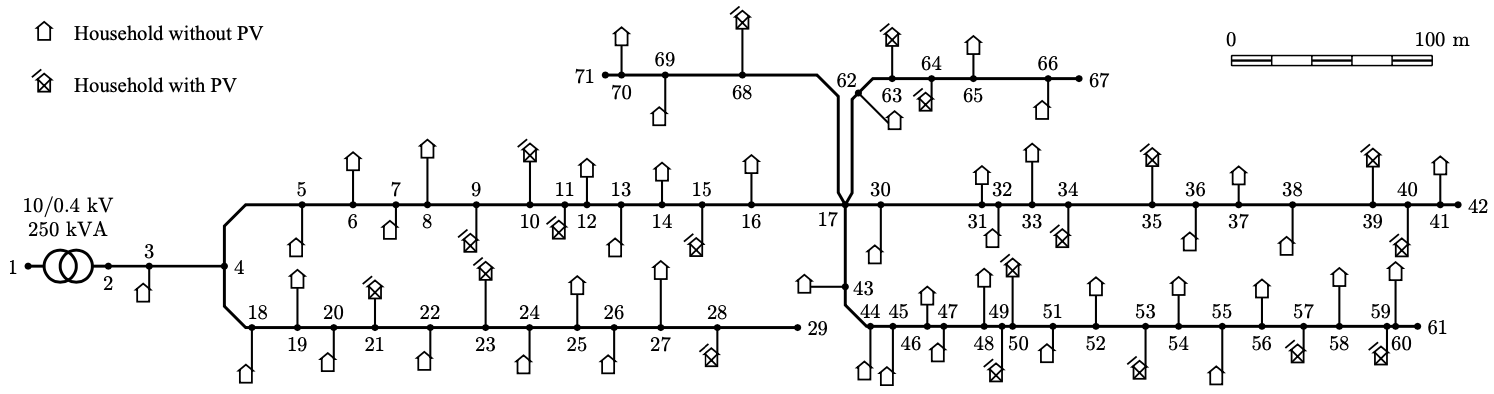
\includegraphics{../Pictures/case70true.png}

\begin{itemize}
\tightlist
\item
  located in Belgium.
\item
  one step-down transformer between bus 1 and bus 2 (not considered)
\item
  bus 1 is omitted
\item
  three-phase four-wire cables
\item
  one phase star connection
\item
  Houses associated with buses 3, 7, 10, 13, 16, 20, 23, 26, 30, 33, 36, 39,
  43, 46, 49, 52, 55, 58, 62, 65, 69 are connected through phase A.
\item
  Houses associated with buses 5, 8, 11, 14, 18, 21, 24, 27, 31, 34, 37, 40,
  44, 47, 50, 53, 56, 59, 63, 66, 70 are connected through phase B.
\end{itemize}

\hypertarget{power-flow}{%
\chapter{Power Flow}\label{power-flow}}

  \bibliography{bibliography.bib}

\end{document}
